\documentclass[journal,12pt,twocolumn]{IEEEtran}
\usepackage{setspace}
\usepackage{gensymb}
\usepackage{caption}
%\usepackage{multirow}
%\usepackage{multicolumn}
%\usepackage{subcaption}
%\doublespacing
\singlespacing
\usepackage{csvsimple}
\usepackage{amsmath}
\usepackage{multicol}
%\usepackage{enumerate}
\usepackage{amssymb}
%\usepackage{graphicx}
\usepackage{newfloat}
%\usepackage{syntax}
\usepackage{listings}
\usepackage{color}
\usepackage{tikz}
\usepackage{graphicx}
\usetikzlibrary{shapes,arrows}

%\usepackage{graphicx}
%\usepackage{amssymb}
%\usepackage{relsize}
%\usepackage[cmex10]{amsmath}
%\usepackage{mathtools}
%\usepackage{amsthm}
%\interdisplaylinepenalty=2500
%\savesymbol{iint}
%\usepackage{txfonts}
%\restoresymbol{TXF}{iint}
%\usepackage{wasysym}
\usepackage{amsthm}
\usepackage{mathrsfs}
\usepackage{txfonts}
\usepackage{stfloats}
\usepackage{cite}
\usepackage{cases}
\usepackage{mathtools}
\usepackage{caption}
\usepackage{enumerate}	
\usepackage{enumitem}
\usepackage{amsmath}
%\usepackage{xtab}
\usepackage{longtable}
\usepackage{multirow}
%\usepackage{algorithm}
%\usepackage{algpseudocode}
\usepackage{enumitem}
\usepackage{mathtools}
\usepackage{hyperref}
%\usepackage[framemethod=tikz]{mdframed}
\usepackage{listings}
    %\usepackage[latin1]{inputenc}                                 %%
    \usepackage{color}                                            %%
    \usepackage{array}                                            %%
    \usepackage{longtable}                                        %%
    \usepackage{calc}                                             %%
    \usepackage{multirow}                                         %%
    \usepackage{hhline}                                           %%
    \usepackage{ifthen}                                           %%
  %optionally (for landscape tables embedded in another document): %%
    \usepackage{lscape}     


\usepackage{url}
\def\UrlBreaks{\do\/\do-}


%\usepackage{stmaryrd}


%\usepackage{wasysym}
%\newcounter{MYtempeqncnt}
\DeclareMathOperator*{\Res}{Res}
%\renewcommand{\baselinestretch}{2}
\renewcommand\thesection{\arabic{section}}
\renewcommand\thesubsection{\thesection.\arabic{subsection}}
\renewcommand\thesubsubsection{\thesubsection.\arabic{subsubsection}}

\renewcommand\thesectiondis{\arabic{section}}
\renewcommand\thesubsectiondis{\thesectiondis.\arabic{subsection}}
\renewcommand\thesubsubsectiondis{\thesubsectiondis.\arabic{subsubsection}}

% correct bad hyphenation here
\hyphenation{op-tical net-works semi-conduc-tor}

%\lstset{
%language=C,
%frame=single, 
%breaklines=true
%}

%\lstset{
	%%basicstyle=\small\ttfamily\bfseries,
	%%numberstyle=\small\ttfamily,
	%language=Octave,
	%backgroundcolor=\color{white},
	%%frame=single,
	%%keywordstyle=\bfseries,
	%%breaklines=true,
	%%showstringspaces=false,
	%%xleftmargin=-10mm,
	%%aboveskip=-1mm,
	%%belowskip=0mm
%}

%\surroundwithmdframed[width=\columnwidth]{lstlisting}
\def\inputGnumericTable{}                                 %%
\lstset{
%language=C,
frame=single, 
breaklines=true,
columns=fullflexible
}

\begin{document}
%
\tikzstyle{block} = [rectangle, draw,
    text width=3em, text centered, minimum height=3em]
\tikzstyle{sum} = [draw, circle, node distance=3cm]
\tikzstyle{input} = [coordinate]
\tikzstyle{output} = [coordinate]
\tikzstyle{pinstyle} = [pin edge={to-,thin,black}]

\theoremstyle{definition}
\newtheorem{theorem}{Theorem}[section]
\newtheorem{problem}{Problem}
\newtheorem{proposition}{Proposition}[section]
\newtheorem{lemma}{Lemma}[section]
\newtheorem{corollary}[theorem]{Corollary}
\newtheorem{example}{Example}[section]
\newtheorem{definition}{Definition}[section]
%\newtheorem{algorithm}{Algorithm}[section]
%\newtheorem{cor}{Corollary}
\newcommand{\BEQA}{\begin{eqnarray}}
\newcommand{\EEQA}{\end{eqnarray}}
\newcommand{\define}{\stackrel{\triangle}{=}}
\bibliographystyle{IEEEtran}
%\bibliographystyle{ieeetr}
\providecommand{\nCr}[2]{\,^{#1}C_{#2}} % nCr
\providecommand{\nPr}[2]{\,^{#1}P_{#2}} % nPr
\providecommand{\mbf}{\mathbf}
\providecommand{\pr}[1]{\ensuremath{\Pr\left(#1\right)}}
\providecommand{\qfunc}[1]{\ensuremath{Q\left(#1\right)}}
\providecommand{\sbrak}[1]{\ensuremath{{}\left[#1\right]}}
\providecommand{\lsbrak}[1]{\ensuremath{{}\left[#1\right.}}
\providecommand{\rsbrak}[1]{\ensuremath{{}\left.#1\right]}}
\providecommand{\brak}[1]{\ensuremath{\left(#1\right)}}
\providecommand{\lbrak}[1]{\ensuremath{\left(#1\right.}}
\providecommand{\rbrak}[1]{\ensuremath{\left.#1\right)}}
\providecommand{\cbrak}[1]{\ensuremath{\left\{#1\right\}}}
\providecommand{\lcbrak}[1]{\ensuremath{\left\{#1\right.}}
\providecommand{\rcbrak}[1]{\ensuremath{\left.#1\right\}}}
\theoremstyle{remark}
\newtheorem{rem}{Remark}
\newcommand{\sgn}{\mathop{\mathrm{sgn}}}
\providecommand{\abs}[1]{\left\vert#1\right\vert}
\providecommand{\res}[1]{\Res\displaylimits_{#1}} 
\providecommand{\norm}[1]{\left\Vert#1\right\Vert}
\providecommand{\mtx}[1]{\mathbf{#1}}
\providecommand{\mean}[1]{E\left[ #1 \right]}
\providecommand{\fourier}{\overset{\mathcal{F}}{ \rightleftharpoons}}
%\providecommand{\hilbert}{\overset{\mathcal{H}}{ \rightleftharpoons}}
\providecommand{\system}{\overset{\mathcal{H}}{ \longleftrightarrow}}
	%\newcommand{\solution}[2]{\textbf{Solution:}{#1}}
\newcommand{\solution}{\noindent \textbf{Solution: }}
\newcommand{\myvec}[1]{\ensuremath{\begin{pmatrix}#1\end{pmatrix}}}
\providecommand{\dec}[2]{\ensuremath{\overset{#1}{\underset{#2}{\gtrless}}}}
\DeclarePairedDelimiter{\ceil}{\lceil}{\rceil}
%\numberwithin{equation}{section}
%\numberwithin{problem}{subsection}
%\numberwithin{definition}{subsection}
\makeatletter
\@addtoreset{figure}{section}
\makeatother
\let\StandardTheFigure\thefigure
%\renewcommand{\thefigure}{\theproblem.\arabic{figure}}
\renewcommand{\thefigure}{\thesection}
%\numberwithin{figure}{subsection}
%\numberwithin{equation}{subsection}
%\numberwithin{equation}{section}
%\numberwithin{equation}{problem}
%\numberwithin{problem}{subsection}
\numberwithin{problem}{section}
%%\numberwithin{definition}{subsection}
%\makeatletter
%\@addtoreset{figure}{problem}
%\makeatother
\makeatletter
\@addtoreset{table}{section}
\makeatother
\let\StandardTheFigure\thefigure
\let\StandardTheTable\thetable
\let\vec\mathbf
\numberwithin{equation}{section}
\vspace{3cm}
\title{%Convex Optimization in Python
	Random Numbers
}
%\title{
%	\logo{Matrix Analysis through Octave}{\begin{center}\includegraphics[scale=.24]{tlc}\end{center}}{}{HAMDSP}
%}
% paper title
% can use linebreaks \\ within to get better formatting as desired
%\title{Matrix Analysis through Octave}
%
%
% author names and IEEE memberships
% note positions of commas and nonbreaking spaces ( ~ ) LaTeX will not break
% a structure at a ~ so this keeps an author's name from being broken across
% two lines.
% use \thanks{} to gain access to the first footnote area
% a separate \thanks must be used for each paragraph as LaTeX2e's \thanks
% was not built to handle multiple paragraphs
%
\author{Mannem Charan - AI21BTECH11019}
\maketitle
\tableofcontents
\bigskip
\renewcommand{\thefigure}{\theenumi}
\renewcommand{\thetable}{\theenumi}

\begin{abstract}
This manual provides solutions for random numbers assignment.
\end{abstract}
%%
\section{Uniform Random Numbers}
Let $U$ be a uniform random variable between 0 and 1.
\begin{enumerate}[label=\thesection.\arabic*,ref=\thesection.\theenumi]
\item Generate $10^6$ samples of $U$ using a C program and save into a file called uni.dat .
\\
\solution Download the following files.
\begin{lstlisting}
wget https://github.com/Charanyash/Random-Numbers-/blob/main/codes/uniform.c 
wget https://github.com/Charanyash/Random-Numbers-/blob/main/codes/coeffs.h
\end{lstlisting}
Then use the following commands in linux terminal,
\begin{lstlisting}
cc uniform.c -lm
./a.out
\end{lstlisting}

%
\item
Load the uni.dat file into python and plot the empirical CDF of $U$ using the samples in uni.dat. The CDF is defined as
\begin{align}
F_{U}(x) = \pr{U \le x}
\end{align}
\\
\solution  Use the following code to plot Fig. \ref{fig:uni_cdf}
\begin{lstlisting}
wget https://github.com/Charanyash/Random-Numbers-/blob/main/codes/uniform_cdf_plot.py
\end{lstlisting}
Run the following command in the linux terminal,
\begin{lstlisting}
python3 uniform_cdf_plot.py
\end{lstlisting}

\begin{figure}
\centering
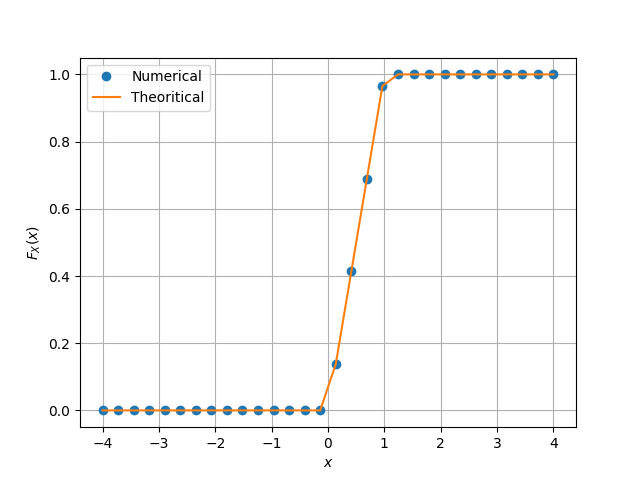
\includegraphics[width=\columnwidth]{figs/uni_cdf.png}
\caption{The CDF of $U$}
\label{fig:uni_cdf}
\end{figure}

%
\item
Find a  theoretical expression for $F_{U}(x)$.
\solution Given that, random variable $U$ is uniformly distributed in interval $\brak{0,1}$ . So we can write that, the probability density function
               \begin{align}
                        f_{x}\brak{x} &= \frac{1}{1 -0}\\
                                      &= 1
               \end{align}
       So for $ U \in \brak{0,1} $ , the probability distribution function $F_{x}\brak{x}$ can be calculated as,
               \begin{align}
                           F_{x}\brak{x} &= \int_{0}^{x} f_x\brak{x}dx\\
                                         &= \int_{0}^{x}1dx\
                                         &= x
                \end{align}

            Since $U$ is distributed from 0 to 1, we can write
		\begin{equation*}
                                 F_{x}\brak{x} = \begin{cases}
                                                          0  &, x \leq 0 \\
                                                          x  &, 0<x<1 \\
                                                          1  & , x \geq 1
                                                        \end{cases}
                 \end{equation*}

\item
The mean of $U$ is defined as
%
\begin{equation}
E\sbrak{U} = \frac{1}{N}\sum_{i=1}^{N}U_i
\end{equation}
%
and its variance as
%
\begin{equation}
\text{var}\sbrak{U} = E\sbrak{U- E\sbrak{U}}^2 
\end{equation}

Write a C program to  find the mean and variance of $U$. 
\solution Download the following code,
 \begin{lstlisting}
wget https://github.com/Charanyash/Random-Numbers-/blob/main/codes/mean_var_uniform.c
wget https://github.com/Charanyash/Random-Numbers-/blob/main/codes/coeffs.h
 \end{lstlisting}
Run the following command,
 \begin{lstlisting}
cc mean_var_uniform.c -lm
./a.out
 \end{lstlisting}
We will get output as,
\begin{align}
	mean &= 0.500007\\
     variance&= 0.083301
\end{align}
	
\item Verify your result theoretically given that
\end{enumerate}
%
\begin{equation}
E\sbrak{U^k} = \int_{-\infty}^{\infty}x^kdF_{U}(x)
\end{equation}
\solution Already we know that,
                \begin{equation*}
                                 F_{x}\brak{x} = \begin{cases}
                                                          0  &, x \leq 0 \\
                                                          x  &, 0<x<1 \\
                                                          1  & , x \geq 1
                                                        \end{cases}
                 \end{equation*}

So, the given integral solves down to,
 \begin{equation}
	 E\sbrak{U^k} = \int_{0}^{1}x^kdx
 \end{equation}
Since $F_{x}\brak{x}$ is constant w.r.t x for $ x \geq 1 $ amd $ x \leq 0 $.\\
For mean,
  \begin{align}
	  E\sbrak{U} &= \int_{0}^{1}xdx\\
	             &=\cbrak{ \frac{x^{2}}{2}}_{0}^{1} 
              &= 0.5
  \end{align}
Now for variance,we know that
  \begin{align}
	  Var\sbrak{U} &= E\sbrak{U- E\sbrak{U}}^2 \\
		       &= E\sbrak{U^{2} + E\sbrak{U}^{2} - 2E\sbrak{U}U}\\
		       &= E\sbrak{U^{2}} + E\sbrak{U}^{2} - 2E\sbrak{U}^{2}\\
		       &= E\sbrak{U^{2}} - E\sbrak{U}^{2} \label{eq:1-8}
  \end{align}
And 
  \begin{align}
	  E\sbrak{U^{2}} &= \int_{0}^{1}x^{2}dx\\
			 &=\cbrak{ x^{3}/3}_{0}^{1}
			 &= \frac{1}{3}
  \end{align}
  Therefore,
  \begin{align}
	  Var\sbrak{U} &= \frac{1}{3} -\brak{ \frac{1}{2}}^{2}
		       &= \frac{1}{3} - \frac{1}{4}
		       &= \frac{1}{12}
		       &= 0.0833
  \end{align}
\section{Central Limit Theorem}
%
\begin{enumerate}[label=\thesection.\arabic*
,ref=\thesection.\theenumi]

%
\item
Generate $10^6$ samples of the random variable
%
\begin{equation}
X = \sum_{i=1}^{12}U_i -6
\end{equation}
%
using a C program, where $U_i, i = 1,2,\dots, 12$ are  a set of independent uniform random variables between 0 and 1
and save in a file called gau.dat
\solution Download the code below

\begin{lstlisting}
wget https://github.com/Charanyash/Random-Numbers-/blob/main/codes/gaussian.c
wget https://github.com/Charanyash/Random-Numbers-/blob/main/codes/coeffs.h
\end{lstlisting}
Run the following command
\begin{lstlisting}
cc  gaussian.c
./a.out
\end{lstlisting}
 
%
\item
Load gau.dat in python and plot the empirical CDF of $X$ using the samples in gau.dat. What properties does a CDF have?
\\
\solution Download the below code,
\begin{lstlisting}
wget https://github.com/Charanyash/Random-Numbers-/blob/main/codes/gaussian_cdf_plot.py
\end{lstlisting}
Run the following command to get CDF plot,
\begin{lstlisting}
python3 gaussian_cdf_plot.py
\end{lstlisting}
The CDF of $X$ is plotted in Fig. \ref{fig:gauss_cdf}.\\
\textbf{Properties Of CDF:}
 \begin{enumerate}
	 \item $ F_{X}\brak{x} = P(X \leq x)= \frac{1}{\sqrt{2\pi}}\int_{-\infty}^{x}\exp\brak{-\frac{x^2}{2}}dx$.
	 \item $ \lim \limits_{x\rightarrow \infty} F_{x}\brak{x}=1, \hspace{5pt} \lim \limits_{x\rightarrow -\infty} F_{x}\brak{x}=0$
	 \item $ F_{X}\brak{x} = \frac{1}{2}$
	 \item $ F_{X}\brak{-x} = 1 - F_{X}\brak{x} $		 
 \end{enumerate}

\begin{figure}
\centering
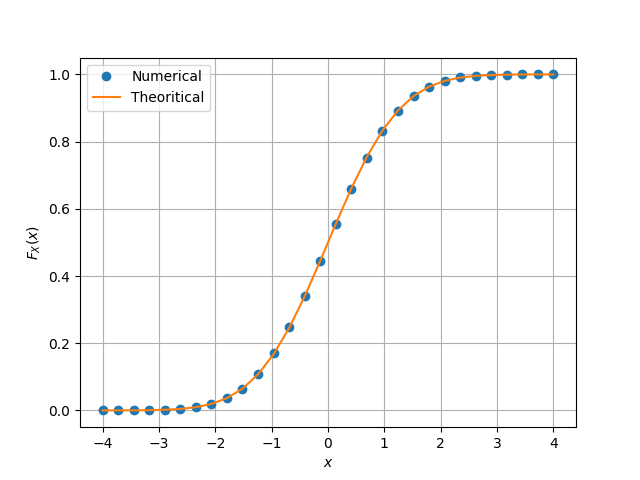
\includegraphics[width=\columnwidth]{figs/gauss_cdf.png}
\caption{The CDF of $X$}
\label{fig:gauss_cdf}
\end{figure}
\item
Load gau.dat in python and plot the empirical PDF of $X$ using the samples in gau.dat. The PDF of $X$ is defined as
\begin{align}
p_{X}(x) = \frac{d}{dx}F_{X}(x)
\end{align}
What properties does the PDF have?\\
\solution The PDF of $X$ is plotted in Fig. \ref{fig:gauss_pdf} using the code below
\begin{lstlisting}
wget https://github.com/Charanyash/Random-Numbers-/blob/main/codes/gaussian_pdf_plot.py
\end{lstlisting}
Run the following command,
\begin{lstlisting}
python3 gaussian_pdf_plot.py
\end{lstlisting}
\begin{figure}
\centering
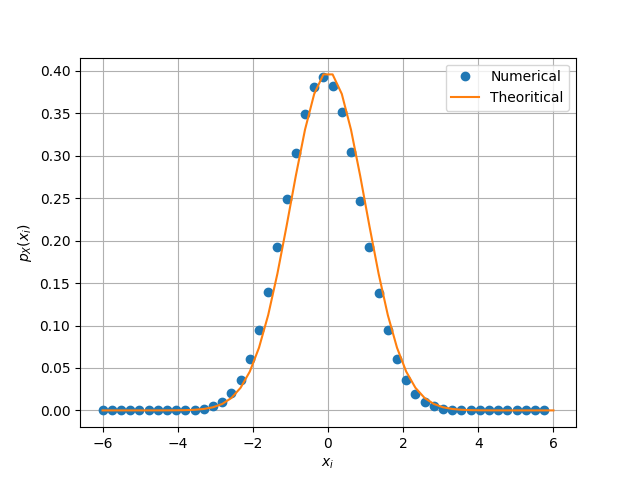
\includegraphics[width=\columnwidth]{figs/gauss_pdf.png}
\caption{The PDF of $X$}
\label{fig:gauss_pdf}
\end{figure}
\textbf{Properties of PDF:}
\begin{enumerate}
     \item PDF is symmetric about the mean, in this case at $x=0$
     \item It has bell shaped graph.
     \item The maxima of the curve is observed at mean of distribution.
\end{enumerate}	     

\item Find the mean and variance of $X$ by writing a C program.
\solution Download the C code from the links below,
\begin{lstlisting}
wget https://github.com/Charanyash/Random-Numbers-/blob/main/codes/mean_var_gauss.c
wget https://github.com/Charanyash/Random-Numbers-/blob/main/codes/coeffs.h
\end{lstlisting}
Then run the following command in linux terminal
\begin{lstlisting}
cc mean_var_gauss.c -lm
./a.out
\end{lstlisting}
we will get $mean = 0.000326, variance = 1.000906$
\item Given that 
\begin{align}
p_{X}(x) &= \frac{1}{\sqrt{2\pi}}\exp\brak{-\frac{x^2}{2}}, -\infty < x < \infty,
\end{align}
repeat the above exercise theoretically.
\solution Given that,
 \begin{align}
p_{X}(x) &= \frac{1}{\sqrt{2\pi}}\exp\brak{-\frac{x^2}{2}}, -\infty < x < \infty,
 \end{align} 
 We know that,
   \begin{align}
	   E\sbrak{x} &= \int_{-\infty}^{\infty}xp_{X}\sbrak{x}dx\\
	              &= \int_{-\infty}^{\infty}\frac{1}{\sqrt{2\pi}}\exp\brak{-\frac{x^2}{2}}dx
   \end{align}
 Since $\frac{1}{\sqrt{2\pi}}\exp\brak{-\frac{x^2}{2}}$ is an odd function.We can write,
   \begin{align}
	   E\sbrak{x} &= 0 \label{eq:2-3}
   \end{align}
 Consider the following expression,
   \begin{align}
	   E\sbrak{x^{2}} &= \int_{-\infty}^{\infty}x^{2}p_{X}\sbrak{x}dx\\
	                  &=\frac{1}{\sqrt{2\pi}}\int_{-\infty}^{\infty}x^{2}e^{\brak{-\frac{x^2}{2}}}dx
   \end{align}
To solve the above integral, we will use integration by parts, i.e,\\
  \begin{align}
	  \int uvdx &= u\int vdx -\int\brak{ u'\brak{\int v}}dx  \\
	  E\sbrak{x^{2}} &= \frac{1}{\sqrt{2\pi}}\brak{\int_{-\infty}^{\infty}x\brak{xe^{-\frac{x^2}{2}}}dx}\\
			         &= \frac{1}{\sqrt{2\pi}}\brak{x\int x e^{-\frac{x^2}{2}}dx -  \int\brak{\int e^{-\frac{x^2}{2}}dx}}
  \end{align}
For the integral $\int x\exp\brak{-\frac{x^2}{2}}dx$ let us take,
  \begin{align}
	   t &= \frac{x^2}{2}\\
	  dt &= xdx\\
	  \int x\exp\brak{-\frac{x^2}{2}}dx &= \int\exp\brak{-t}dt\\
					                &=  -\exp\brak{-t} + c \\
				          \implies  &= -\exp\brak{-\brak{\frac{x^{2}}{2}}} + c \label{eq:2-6}
  \end{align}
 Using \eqref{eq:2-6},we can write
  \begin{align}
	  E\sbrak{x^{2}} &= \frac{1}{\sqrt{2\pi}}\brak{ -xe^{\brak{-\frac{x^{2}}{2}}} + \int e^{\brak{\frac{-x^{2}}{2}}}dx}
  \end{align}
  And we know that,
  \begin{align}
	  \frac{1}{\sqrt{2\pi}}\int_{-\infty}^{\infty}e^{\brak{\frac{-x^{2}}{2}}} &= 1 \label{eq:2-8}
  \end{align}
 Now putting limits and using \eqref{eq:2-3},\eqref{eq:2-8},
  \begin{align}
     E\sbrak{x^{2}} &= 1
  \end{align}	  
Using \eqref{eq:1-8} we can write,
   \begin{align}
    Var\sbrak{x} &= 1 - 0\\
	               &= 1
   \end{align}                           
%
\end{enumerate}
\section{From Uniform to Other}
\begin{enumerate}[label=\thesection.\arabic*,ref=\thesection.\theenumi]
%
\item
Generate samples of 
%
\begin{equation}
V = -2\ln\brak{1-U}
\end{equation}
%
and plot its CDF.
\solution Download the C code from the link below to generate samples of V from uni.dat file
\begin{lstlisting}
wget  https://github.com/Charanyash/Random-Numbers-/blob/main/codes/V.c
\end{lstlsiting}
Run the following command,
\begin{lstlisting}
cc rayleigh.c -lm
./a.out
\end{lstlisting}
Then download the below python file get CDF
\begin{lstlisting}
wget https://github.com/Charanyash/Random-Numbers-/blob/main/codes/V_cdf_plot.py
\end{lstlisting}
Then run the following command
\begin{lstlisting}
python3 rayleigh_cdf_plot.py
\end{lstlisting}
\begin{figure}
\centering
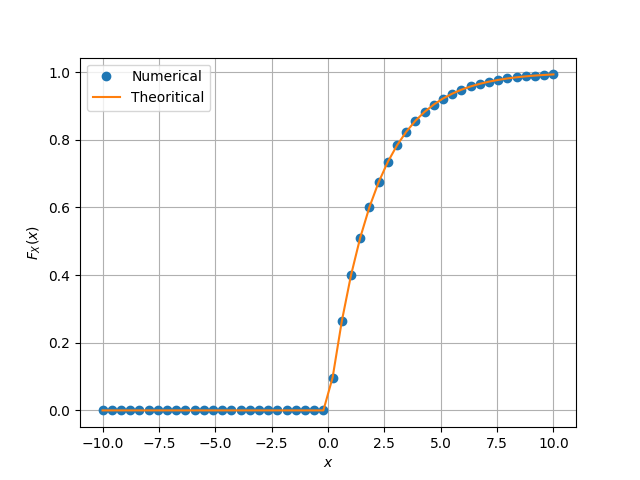
\includegraphics[width=\columnwidth]{figs/V_cdf.png}
\caption{The CDF of $V$}
\label{fig:V_cdf}
\end{figure}

\item Find a theoretical expression for $F_V(x)$.
\solution Given 
\begin{align}
	V &= -2\ln\brak{1-U} \label{eq: 3-2}
\end{align}
 For, 
 \begin{align}
	 F_V\brak{x} &= \pr{V\leq x}
 \end{align}
 we will use \eqref{eq:3-2}
 \begin{align}
	 F_V\brak{x} &= \pr{-2\ln\brak{1-U} \leq x}\\
	             &= \pr{ \ln\brak{1-U} \geq \frac{-x}{2}}\\
		           &= \pr{  1-U \geq \exp\brak{\frac{-x}{2}}}\\
		           &= \pr{ U \leq 1 - \exp\brak{\frac{-x}{2}}}\\
               &= F_U\brak{1-\exp\brak{\frac{-x}{2}}}\\
 \end{align}
 Using CDF of U,
 \begin{equation*}
         F_{x}\brak{x} = \begin{cases}
                            0  &, x < 0 \\
                            1 - e^{frac{-x}{2}}  &, x\geq 0 
                         \end{cases}
\end{equation*}


%
%\item
%Generate the Rayleigh distribution from Uniform. Verify your result through graphical plots.
\end{enumerate}


\end{document}
